\documentclass[12pt,a4paper,finnish]{assets/tutthesis}
 
% LaTeX-tiedosto opinnäytepohjaksi
% Tekijä: Sami Paavilainen
% Muokkaaja: Heikki Huttunen (heikki.huttunen@tut.fi) 31.7.2012.
% Lisämuokkaajat: Mikko Pohja & Miro Nieminen ~2014
 
% Vaatii lisäksi luokkatiedoston tutthesis.cls
% sekä tiedoston tty-logo.pdf (pdflatex) tai tty-logo-eps (latex)

\usepackage[utf8]{inputenc}

% kuvatekstien kirjasinkoko ja asettelu
\usepackage[small]{caption}

% koodilistauksia varten tarvittavat hässäkät
\usepackage{listings}
\captionsetup[lstlisting]{ format=listing, labelfont=white, textfont=white, singlelinecheck=false, margin=0pt, font={bf,footnotesize} }


% omia käskyjä voi lisätä tähän väliin, esim. \newcommand{\angs}{\textsl{\AA}}

\pagenumbering{Roman}

% // alkuvalmistelut loppuu


% Tästä alkaa varsinainen teksti
\begin{document}
\thispagestyle{empty}
 
\vspace*{-.5cm}\noindent
 
% If thesis is in English, use the file "tut-logo"
% instead of "tty-logo" in the following:
 

\includegraphics[width=8cm]{assets/tut-logo}
 
\vspace{6.8cm}
 
\noindent{\bf\large \textsf{Miro Nieminen}}\\
{\bf\large \textsf{Fallback Mechanisms for Connection Loss in Single-Page Web Applications}}\\
\textsf{Master of Science Thesis}
 
\vspace{8.7cm} % jos kaksi otsikkoriviä vaihda -> 6.7cm
 
\begin{flushright}
  
\begin{minipage}[c]{6.8cm}
\begin{spacing}{1.0}
\textsf{Examiners: Tommi Mikkonen}\\
\textsf{Examiners and topic approved in}\\ 
\textsf{the Information Technology}\\
\textsf{Department Council meeting on}\\
\textsf{xx.xx.xxxx}\\
\end{spacing}
\end{minipage}
\end{flushright}



%% ----------------------------------------
\newpage
 
\setcounter{page}{1} % tämä tarvitaan, jottei ensimmäinen sivu kansilehden jälkeen olisi numero 2.
 
\chapter*{TIIVISTELMÄ}
\begin{spacing}{1.0}
\textsf{TAMPEREEN TEKNILLINEN YLIOPISTO}\\
\textsf{Tietotekniikan koulutusohjelma}\\
{\bf \textsf{Miro Nieminen: Fallback Mechanisms for Connection Loss in Single-Page Web Applications}}\\
\textsf{Diplomityö, xx sivua}\\
\textsf{Xxxxxkuu 2015}\\
\textsf{Pääaine: }\\
\textsf{Tarkastajat: Tommi Mikkonen}\\
\textsf{Avainsanat: JavaScript, Single-Page Application, Computer Supported Collaborative Work, Offline Support}\\
\end{spacing}
 
\noindent
Tekstiä
 
\noindent
Tekstiä





%% ----------------------------------------
\newpage
\chapter*{ABSTRACT}
\begin{spacing}{1.0}
\textsf{TAMPERE UNIVERSITY OF TECHNOLOGY}\\
\textsf{Master's Degree Programme in Information Technology}\\
{\bf \textsf{Miro Nieminen: Fallback Mechanisms for Connection Loss in Single-Page Web Applications}}\\
\textsf{Master of Science Thesis, xx pages}\\
\textsf{xxxxxx 2015}\\
\textsf{Major: }\\
\textsf{Examiner: Tommi Mikkonen}\\
\textsf{Keywords: JavaScript, Single-Page Application, Computer Supported Collaborative Work, Offline Support}\\
\end{spacing}
 
 % Konteksti
\noindent
Here will be dragons
 
 % Ongelma
\noindent

 % Tässä diplomityössä (mitä tehty ratkaisemiseksi)
\noindent

% Arvio onnistumisesta
\noindent




%% ----------------------------------------
\newpage
 
\chapter*{PREFACE}
\noindent 

Your advertisement could be here.




%% ----------------------------------------
\newpage
\tableofcontents
%\newpage
%\listoffigures
%\listoftables






%% ----------------------------------------
% \newpage
% \chapter*{TERMS AND DEFINITIONS}
%  
% % Näitä ei välttämättä tarvi olla
% \begin{termiluettelo}
%  
% \item [Life cycle] TODO
% \item [Function point] TODO
%  
% \end{termiluettelo} 
 



%% ----------------------------------------
\newpage
\renewcommand{\chaptermark}[1]{\markboth{\thechapter. \ #1}{}}
\renewcommand{\sectionmark}[1]{\markright{}{}}
\lhead{\fancyplain{}{\leftmark}}
 

\pagenumbering{arabic}
 

%% ---------------------------------------
%% Introduction
\chapter{Introduction}
%% TODO:
% -pähkinänkuoressa koko setti tänne!



% ### yleistä taustaa (esim. on enemmän ja enemmän verkon kautta käytettäviä mobiilipalveluita. tämä vaatii sen että verkko toimii, ihmisten arki ja sen vuorovaikutustilanteen ovat nykyään hyvin verkkovälitteisiä)
% Maailma digitalisoituu ympärillämme, yhä useampi työtehtävistä ja vapaa-ajan aktiviteeteista liittyy jotenkin digitaalisiin palveluihin ja laitteisiin. Harva näistä toimii täysin ilman Internetin tukea
The world is digitalizing around us on a always more quicker pace. More and more of our work tasks and our past time activities are somehow affiliated to digital devices and services. Most of these things are often useless without connectivity to a broader context, usually the Internet. 

% Mobile usage has surpassed desktop usage in <lähde>, on jo iso joukko käyttäjiä joiden ainoa tie Internetiin on heidän mobiililaitteensa <lähde>. Joku viittaus "seuraavaan miljardiin netin käyttäjään?""
Age of the desktop hegemony is already over. XX percentage of people use mobile devices as their primary method of accessing the Internet. <viite> Unlike as in desktop devices, which usually are operated from static location aided by cable access to the Internet, mobile devices often travel with their owners where ever they might go. That creates challenges for connectivity, which is nowadays essentials for device proper usage. 

% Mobiilinetti-coverage ei optimaalinen -> verkkokatkoksia tulee, laadullisia ja kokonaan yhteyden katoamisia. Näiltä ei voida välttyä.
When mobile device is not in the coverage area of an Wireless Local Area Network, device relies on mobile broadband connection. Mobile broadband coverage varies within different locations. When moving away from the nearest base station the reception of signal weakens. Mobile device user experiences this as an increased latency times, lower data transferring speeds, or even as a total blackout of the broadband service. When moving away from highly populated areas this is unevitable, since not all locations are to be covered properly while keeping cost efficiency on a sane level <source?>, especially in countries with large acreage but low population, like Finland. However digitalization of services is even more important on a places like this, since supplying physical services to areas with low population density is expensive. 

People are more and more reliant digital services and their device of choose is mobile devices on an increasing scale. But how to use services and devices dependent on the Internet with coincidental connection? The thesis you are about to read researches this problem. 

% Tämä dippa tarkastelee tätä perusyhtälöä ohjelmistonkehittäjän kannalta - kuinka ja millä tasolla verkon laadun huonontumiseen/kokonaiseen katkeamiseen tulisi varautua? Onko mahdollista abstarhoida verkon laadun vaihteleminen käyttäjältä piiloon kokonaan, ja hallita sen tuomat ongelmat applikaation sisäisesti? Millaisia resursseja tällainen vaatii ohjelmiston kehitysvaiheessa? Entä mahdollinen lisäkuorma laitteille?



\section{Research Objectives}
The objective of this research is to find useful and working fallback mechanisms for connectivity loss in Single-Page Web Applications, in both from the user experience perspective and from the developer's viewpoint. The state where the application loses the connectivity to the Internet is referred on this thesis as an \textbf{offline mode}. This thesis tries to find efficient methods of allowing the user to continue his/hers tasks when the connection is lost and the application enters the offline mode.

From software development point of view looking, how to deliver seamless user experience, even when the connectivity is bad or nonexistent? How much resources can this reserve on the development phase? Is it possible to abstract the connection quality completely away and handle the issues with connection internally on the application level, invisible to the user?

From the user experience perspective, how to notify the user about the loss of Internet connection? Does the user has to be notified at all? If the user is notified, what is exactly the message that needs to be told? 


This thesis studies one real-life case of implementing offline supported functionality to already existing system created for supporting daycare personnel and the parents of daycare children, the Päikky system. <tähä jotai lisää päikystä>



\section{Research Question}
This thesis answers to the following question: "How to prepare for Internet connection shortages on a Single-Page web application?"
% TODO: block quote for the question

\section{Scope}
The whole Internet is build on top of the client-server -paradigm [Berson]. In this thesis we focus on the client end of this paradigm and research ways of dealing the connectivity problem in there while delimiting the server out of this thesis' context. 

On the client we will focus on how to deal with the issue on the web application level inside the browser environment, ignoring the possible solutions that could be done on the device platform tier. Therefore results of this thesis will apply browsers in desktop computers, tablet devices and mobile phones.


\section{Motivation}
<Yleinen ongelma, saadaan Design Guidelineja aikaiseksi muille kehittäjille, eivät uppoa samoihin kuoppiin kuin mitä me Päikkyä kehittäessä upottiin>


\section{Structure of the thesis}
In here well be described contents of each chapter, because that's how it has always been done.



%% Tommi-input: 
% "rajaus pitää selittää johdannossa,tiivistössä ja abstraktissa"
% -mihin liittyy, konteksti
% -ongelma, mitä tehdään kun yhteys katoaa
% -ratkaisu, “tässä diplomityössä tehdään”
% -arviointi, “miten hyvä tästä tuli”


% HUOM RAJAUS KOSKEMAAN VAIN FRONTEND PÄÄN TEKNIIKOITA
% TUTKIMUSKYSYMYS?!?!?!



% ### - ongelmakentän kuvaus, mikä on tutkimusta vaativa ongelma (kentän katkeaminen ja minkälaisia ongemia se aiheuttaa) ja se ajankohtaisuus ja yleisyys. Ongelma on että ei tiedetä kovin hyvin että kuinka kentän katkeamisen vaikutukset pitäisi ottaa sovelluskehityksessä huomioon niin että käyttäjän tavoitteet sovelluksen käytölle täyttyvät kentän katkeamisesta huolimatta. 






% Tässä dipassa ongelmaa lähdetään selvittämään case studyllä liittyen Päikky-järjestelmään. <Pieni pohjustus järjestelmästä>
% - kerro miten lähdet tässä tutkimuksessa ratkaisemaan ongelmaa. Case tutkimus päiväkotisoftalle. Tehtiin päiväkotisofta, mutta huomattiin että verkonkatkeilu muodostaa merkittävän ongelman (kerro myös konkreettisesti mitä ongelmia katkeilu synnytti). Sitä ongelmaa lähdettiin sitten ratkaisemaan. Softan implementointi ja real life kenttäkoe implementoinnin vaikutuksista 


% <Päikyn ei-offline-versiossa ilmenneet ongelmat>

% <Lyhyesti offline-moden implementoinnista ja tosimaailman kenttäkokeesta>

% Offline-moden vaikutukset käytössä <haastatteluista rojua tähän>

% META:
% pitäisikö intron olla oma kokonaisuus? tarvitsisiko myöhemmissä kappaleissa vielä erikseen avata päikky-järjestelmää, vai voiko introssa käydä perinpohjaisesti läpi päikyn ja sitte that's it? Kävi myös mielessä pitäisikö ennen releated researchia olla yksi kappale nimenomaan Päikky-järjestelmän käytöstä

 

%% ---------------------------------------
%% Background
\chapter{Background}
% "Ongelmakentän esittely".

In this chapter the three prime themes around this thesis are introduced. Basic knowledge of these themes are required in order to fully comprehend all the aspects on the case study investigated on this thesis later on. 

The basics of \textit{web as an application platform} and more precisely the \textit{single-page application} paradigm are introduced as it is the method how the web application is built on the case study. The concept of \textit{computer supported collaborative work} is introduced since the case study's application is essentially that: multiple users collaboratively viewing and editing the same data set. The most usual types of \textit{connectivity issues} and the reasons for them are portrayed, since the disruption created by them to the case study's application created the actual need for offline supported functionalities in the first place. 




%% ----------------------------------
\section{Web Applications}

In the past decade the software industry as a whole has been facing a major paradigm shift on the way how and where applications are developed and operated. Progress in web technologies and standards have made it possible for the browser environment to become a more and more powerful but still universal computing platform. Software applications that were previously built for different kind of operating system and CPU combinations are now written with web technologies and run on the browser. This change is mainly accomplished by the power of distribution the web platform provides. Software provider or the organization's IT function does not have to take care of updating end user software to the latest version anymore, because the client-server paradigm\cite{berson_client-server_1992} makes running outdated software version virtually impossible. In a traditional desktop application patching the software to fix bugs or introducing a new feature requires downloading a installer or a patcher and then it must be run on the computer. This requires action from the user or from the IT function. This might not cover the whole upgrading process in every situation: sometimes updating dependent libraries or operating system might be required. It also enables possibility for different computers to be running different versions of the software, creating circumstances for version mismatches between different clients. \cite{jazayeri_trends_2007} \cite{taivalsaari_mashware:_2009} %[jazayeri 3.3] [taivalsaari_mashware:_2009]

The move from individual installations to a centralized services reverses the general model how software is operated, the model which has been dominating since the start of the personal computing revolution \cite[Chapter 3.3]{jazayeri_trends_2007}. As stated above, this comes with many benefits. One of the most important ones is the (almost) unified platform provided for the developers. Thanks to automatic update mechanisms of the modern browsers, this platform is one of the fastest updating ones there is when it comes to speed of patches applied to end users' computers \cite{duebendorfer_why_2009}. Due to the easiness of the deployment process, it is not unusual to see web application rolling in releases to production on daily or even on hourly basis \cite[Chapter 3.3]{jazayeri_trends_2007}.



% ###
\subsection{Single-Page Applications}
\label{subsec:spa}
% - yleisesti tuotantojavaskriptistä, yks yhdistetty&minimifoitu .js-möykky tuotannossa (tähän viittaan implementaatio-osuudessa)?
% - AMD-moduulin avaus?


Executing complicated applications on the web platform has been made possible by the evolution of the web pages from ``classic'', static presentation consisting of single pages to a more interactive and collaborative web applications. In the early phases of World Wide Web user navigated through hyperlinks within single pages each of them being formed and served by the server. Client, the browser, was responsible only for rendering the response of the server. \cite{taivalsaari_mashware:_2009} The current state of technology allows more of the functionality to be moved or duplicated from the server to the client. When before web pages on the browser were stateless, and the state transforms were done while moving to a new page, now it is possible for the browser to handle the state transitions and retrieve only the needed data from the server when required via AJAX\footnote{Asynchronous JavaScript + XML}-requests. \cite{paulson_building_2005}

Applications following the paradigm described above can be generalized to be \textit{single-page applications}. These kinds of web applications makes a request to the server, and based on the data of the server's response, they form the layout of the page manipulating the browser's \textit{Document Object Model} in real time. This is contrary to the traditional paradigm where based on the client's request the server creates the layout for the data and sends an whole HTML page as a response, and the whole page is refreshed in result. This is also the etymology behind the name of the paradigm: there is no need for user to navigate away from the page, even when the views on the application change.

The application state handling on the browser environment and the increased amount of possibilities on the browser creates the basis for modern web development and the platform for the offline feature: the single-page application. Single-page application is tightly relevant to other hype terms such as \textit{Web 2.0} and the nowadays partly old-fashioned term \textit{DHTML}\footnote{Dynamic HTML}. All single-page applications could be called Web 2.0 applications, but not all Web 2.0 applications are single-page applications. While traditional web pages where synchronously fetched and generated by the web server, single-page application relies on asynchronous pattern on data fetching. \cite{garrett_ajax:_2005} With the asynchronous pattern the browser can fetch resources on smaller chunks when the need arises, usually through REST APIs \cite{masse_rest_2011}. This also makes possible the premise for an \textit{occasionally connected application}, meaning that the web application can function without having a continuous Internet connection \cite{casario_html5_2011}. The application has the ability to fetch data from the API when there is connectivity, and when the connectivity disappears it can function with application logic downloaded to the browser. This widens a lot the range of use cases which can be covered by web applications.



% ###
\subsection{REST APIs}
% - JSON -termin avaus?
% - REST API:sta jotain (Päikky cachettaa nimenomaan tämäntyyppisiä requesteja)\citation{taivalsaari_mashware:_2009}
% - kuva havainnollistamaan että SPA hakee resursseja yksitellen ja vanhassa mallissa haetaan kokonaisia sivuja?
% - tarviikohan AJAXista tänne jotain?

REST is a term first time introduced by \textit{Roy Fielding} in his Ph.D. dissertation \cite{fielding_architectural_2000} as a description for an architecture style of networked systems. The REST acronym stands for \textit{Representational State Transfer}. Even the term REST comes up often in materials relating to web technologies, it has to be remembered that it is more of an idea for architectural style than an actual well-defined standard. 

Roy Fielding explained the term on his dissertation in the following way:
\begin{quote}
	``Representational State Transfer is intended to evoke an image of how a well-designed Web application behaves: a network of web pages (a virtual state-machine), where the user progresses through an application by selecting links (state transitions) resulting in the next page (representing the next state of the application) being transferred to the user and rendered for their use.''
\end{quote}

The momentum behind the wide use of the REST principles rises from the key motivation behind it: REST captures the key components and ideas of which made the Web successful. These characteristics are in use with guiding the evolution of the Web today. \cite{costello_building_2007}

\begin{figure}[t]
\begin{center}
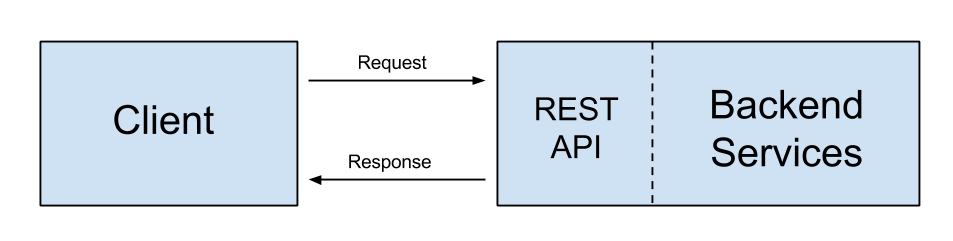
\includegraphics[width=0.8\textwidth]{assets/restapi.png}
\end{center}
\caption{Basic structure of a REST API service, based on the work by Masse \cite{masse_rest_2011}}.
\label{fig:restapi}
\end{figure}

All the single-page applications that interact with data that is used by various clients requires some kind of backend service. Usually this is provided by creating \textit{application programming interfaces} (later on referrenced by APIs) on the backend for the client-server communication. In practice the API exposes methods for fetching and altering the server's data. Therefore APIs can be thought as the \textit{face} for the web service, aimed for listening and responding the clients' requests. \cite{masse_rest_2011}

Figure~\ref{fig:restapi} provides a presentation from Masse~\cite{masse_rest_2011} about the general principle regarding a REST API. Well designed REST API is easily understood by humans, since the URLs themselves should describe precisely what resources will be returned to requests send to them. Using the URLs together with a describing \textit{HTTP method} as a ``verb'' for the operation makes the whole design logical. A REST API can be thought as an assembly of interlinked resources. These resources forms the REST API's \textit{resource model}. \cite{masse_rest_2011}

REST APIs plays an integral part in single-page applications. After the client side code is initialized on the browser, all the actual content (depending on the context whatever that might be) is fetched to the browser via an API which nowadays are almost always RESTful. All the modification and the creation of the data is also done through the functionality exposed to the client by the API. Usually the data is transferred between the client and the server using \textit{JSON objects} (JavaScript Object Notation) for the payload.


% <meta: ajattelin tänne kertoa MVC-mallista ja erityisesti backbonen käyttämästä model-view-template -sovellutuksesta, mutta liekköhän sittenkään oleellista?>

% ###
% \subsection{MVC Architecture}
% - MVT -termin avaus?
% ---> ennen vain view selaimessa, backbonessa koko härveli
% ---> "Frontend gets fatter and fatter" -> Päikyn tilakone myös frontendissä nyt, bisneslogiikka duplikoitava/siirrettävä clienttiin

%[Deacon] -viitteestä löytyy tavaraa tähän jos tarve ilmenee









%% ----------------------------------
\section{Computer Supported Collaborative Work}
% "Reaaliaikaisesta informaationjaosta päiväkotiympäristössä"
% - verkkovälitteinen vuorovaikutus
% - hakusanalla computer supported collaborative work (CSCW) löytyy kamaa 
% - web 2.0 on nimeomaa tätä??

% Käyttämättömien lähteiden lista (löytyvät Zoterosta)


As the automation level of work tasks keeps getting higher, many of the tasks left for human actors on the modern working life gets more complex. The nature of the work also transforms to be much more \textit{distributed} than before, both in the sense of location and time. There is for example a lot more of problem solving and rule interpreting left for the human employees to solve which usually need to be coordinated within the other actors related to that activity. When doing decisions information from several sources have to be considered and noted. \textit{Computer Supported Collaborative Work} (later referred to as CSCW) is a field of study concentrating on how collaborative actions and coordination of them can be aided by support of computer systems. The term was introduced for the first time in 1984 by Irene Greif and Paul M. Cashman. \cite{carstensen_computer_1999}

The Web has been seen as a prolific platform for CSCW implementations since the creation of WWW. The general idea behind WWW by Tim-Berners Lee could be seen as an implementation of a CSCW system. Despite the limitations set by the primitive web technologies of that time, the first implementations of CSCW saw daylight and wide usage already on the 1990's. Usual application for that time concentrated on storing documents on a shared workspace, where a given group could browse and share the documents relating to their work. Even with the limitations set by the web technology that would seem very primitive compared to modern standards, the power of web and ``its ability to provide basic features for cooperation in an integrated service, accessible from different computing platforms and making no demands on users to adopt new word processing, spreadsheet or other application software'' was recognized to be from the highest of potentials. \cite{bentley_basic_1997}

People using CSCW tools can often be described as a group of individuals working synchronously or asynchronously towards of achieving common goal(s). Depending on the situation they can be located on different locations geographically and/or on different time zones. In circumstances such as these all of the people involved have to have up-to-date awareness about each other's intentions, actions and results. \cite{carroll_notification_2003}

From Figure~\ref{fig:cscw-matrix} a reproduced time / space matrix of collaborative systems can be seen based on research done by Saad and Maher \cite{saad_shared_1996}. This matrix splits the types of collaborative systems in to four categories. These categories are not explicitly limited to the CSCW domain but they concern collaboration activities in general. Face to face discussion is the most common case of collaboration happening on same place and time. Traditional physical bulletin boards are an example of collaboration happening on same place different time. Video conference systems are nowadays a common scenario of people from different locations collaborating simultaneously. The evolved Internet version of bulletin boards -- forums and wikis -- can be seen as a way of working from different place and on a different time. That is also the sweet spot for CSCW systems; they deliver the most value to the users when they allow people to collaborate without location or time restrictions. % hox tarvitaanko tänne viite tuon lisäksi vielä? [Saad and Maher]

\begin{figure}[t]
\begin{center}
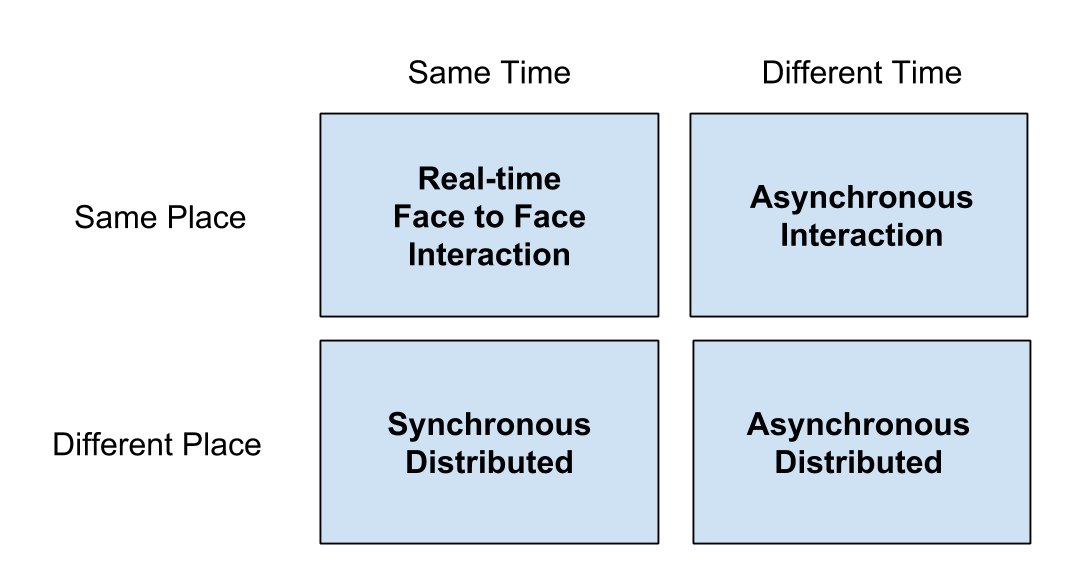
\includegraphics[width=0.8\textwidth]{assets/cscw-matrix.png}
\end{center}
\caption{Collaborative systems in time / space matrix, based on the work by Saad and Maher \cite{saad_shared_1996}.}
\label{fig:cscw-matrix}
\end{figure}


CSCW tools can also be used to create disruption to the hierarchies of the applied work environment, while getting more of the stakeholders involved in the creation of the information. For example in kindergartens the primary gatekeepers for the information flow towards children's homes are the kindergarten nurses. On a research by Näsänen et al. (2009) a web service for showing parents photos taken on the kindergarten were created. One of the goals for the research was to allow efficient way of displaying the life on the kindergarten to the children's parents, whom usually just drop off and pick up the children without being otherwise present. The children also had access to smartphones with camera, allowing them to upload photos directly to the availability of homes without the moderation of kindergarten nurses. \cite{nasanen_mobile_2009}

% The real-life case study of this thesis is essentially an application which provides tools for computer supported collaborative work on kindergarten environment. Awareness of activities and events within the kindergarten are distributed to all the nurses and also to the parents if it concerns their own children. % Tommikommentti: "tätä ei kannata tuoda esiin tipoitellen"







%% ----------------------------------
\section{Connectivity Issues}
% vai pelkkä "Internet Connectivity"?
% http://dl.acm.org/citation.cfm?id=2307649 ?
 % - eri tavat yhdistää internetiin (piuhayhteys, wlan, mobiilidata)
 % - kännyverkon toiminnasta jotain?

 % - kännyverkon toimivuuden vaihtelun yleisyydestä
 % - yleisimmät ongelmatilannetyypit


% Tänne yhdistettynä jotenkin myös vanha "existing methods to solve offline problem" -rojut:
% Minkälaisia offline ratkaisuja on olemassa web/känny-puolella (miten google/microsoft yms. ovat lähestyneet ongelmaa)?
% % onko muita kenttäkokeita tehty offline-moodiin liittyen??

For a single-page application it is possible to work without connection to the outside world, in case the application code is delivered to the device via some medium. For example for a spreadsheet application this might be a highly feasible idea. However for applications that interacts with the surrounding world some kind of connectivity is required in order to spare the person using the system having to input all the data into it. When it comes to CSCW applications, where one of the key points is the \textit{collaboration}, at least occasional Internet connectivity is mandatory. This makes issues on the Internet connectivity status and quality to concern closely CSCW applications. % HOX tää vois toisaalta olla myös ton research gapin rojua? 

In many of the scenarios and application areas where CSCW is applied using desktop computers is challenging or impossible. Often the usage is outlined to the smartphone or/and tablet usage just by the requirement of having the access to the system with the users on all occasions. If the information needs to be accessed immediately on the fly, importable devices are out of the question.

For mobile devices the medium for the ``last mile''\footnote{Metaphor used in telecommunication industry when referring to the part of the network that reaches the customer. When looking from the customer's perspective it can be named as the ``first mile.''} of connecting to the Internet is wirelessly over the radio waves using cellular network. As more and more of the usage of the Internet moves to the mobile devices, the unprecedented cellular traffic growth can easily exceed the deployment speed of cellular infrastructures \cite{qian_web_2012}. This results in a certain \textit{guaranteed unreliability} to the connections of devices using the mobile broadband as their primary method of reaching the Internet. For the time being applications where the possibility of continuous usage is critical bracing oneself to the possible temporary Internet outages is one of the factors which must be taken into account.

One possible solution in overtaking the problems caused by the excess load of cellular networks is to use Wireless LANs as the last mile. With correct configuration this makes the wireless access as reliable as is the Internet connection of the WLAN's base station. However it is not exceptional for a CSCW system to be operated on various locations, resulting in a situation where sometimes usage of cellular network is mandatory. For applications where the SLAs\footnote{Service Level Agreement} are strict and system is used from various locations this method does not deliver any relief.

This thesis studies the issues on the Internet connectivity only from the application level, within the possibilities provided by the browser environment on handling the problem. Possible solutions available on the network-level are ignored.





%% ----------------------------------
\section{Research Gap}
% -> Gappiin ehkä jotain, että verkkovälitteistä vuorovaikutusta on tutkittu paljon (katso CSCW kamaa) ja että mobiiliverkojen tutkimus/kehitys/käyttö ollut räjähdymäistä. Kuitenkaan ei ole paljoa tutkimusta siitä kuinka verkon katkeaminen vaikuttaa reaalisaikaista tiedonvälitystä vaativan sovelluksen käyttökokemukseen ja kuinka sovellussuunnittelussa tulisi katkot ottaa huomioon. 


% This chapter focuses on the background of today's web applications and the literature that relates to the circumstances causing the connectivity issues. This chapter addresses the basics of today's web technologies and the methods that makes offline supported features possible. This chapter coverages also briefly principles on mobile device communication on the network layer, the ideology on Computer Supported Collaborative Work and takes a glimpse on already existing efforts done on solving the offline issue in web applications.  % VANHA INTRO-intro


% "Tämän dipan käsittelemä aihe sijaitsee kolmen edellisen kappaleen keskiössä -> CSCW mahdollistettuna SPA:na mutta Internet-yhteyden katkeamisten riivaamana

\begin{figure}[t]
\begin{center}
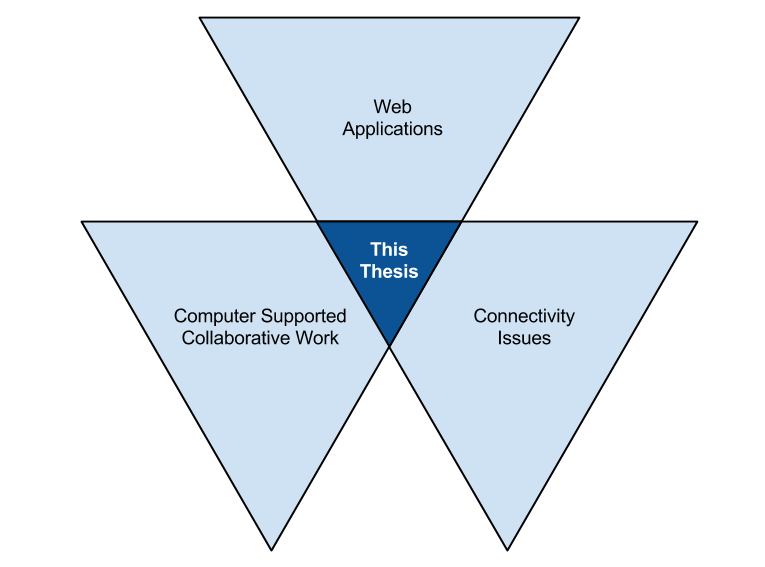
\includegraphics[width=0.8\textwidth]{assets/researchgap.png}
\end{center}
\caption{The research gap covered by this thesis}
\label{fig:researchgap}
\end{figure}

This thesis studies the overlap of the themes previously introduced in this chapter, as can be seen on the visualization in Figure~\ref{fig:researchgap}. This thesis studies what is required from a \textit{single-page application} which enables \textit{computer supported collaborative work} for the users on a environment where \textit{issues with the Internet connectivity} happens regularly. 

CSCW has been studied widely for over the past two decades. The need for streamlining working methods in favor more productivity makes efficient will make applications enabling it only more essential and common.  

The fast-paced evolution of web technologies have created a powerful platform for application development which is ubiquitously present and available everywhere. On the last decade it was available on desktop computers, today it reaches 40~\% of the Earth's population due of increasing usage of mobile devices and tablets \cite{_number_????} and by 2020 \textit{4.9 billion} devices is estimated to be connected\footnote{http://www.gartner.com/newsroom/id/2905717} thanks to the \textit{Internet of Things} (IoT). This will make web technologies only more appealing method for application creation on the future.

With all this taken into account, it would not be surprising if creating applications with the web stack and the need for having an offline support on them would only get more common. Even without the rising need of these kind of applications, the user experience of any web application used over cellular network can be improved significantly with the implementation of a proper offline support, making research around it useful. On top of that there are no existing research covering all of these themes together.









% toistaiseksi hyllytetty kappale, nämä asiat tohon internet connectivity issuesiin messiin
%% ----------------------------------
% \section{Existing Solutions for the Offline Problem}



%% ---------------------------------------
%% Case Päikky

\chapter{Case Päikky}
This thesis approaches the research problem through a real-life case study in which an offline support was implemented to a already existing system. The system under the analysis is \textit{Päikky}, a solution for daycare personnel & daycare children’s parents for planning the needed daycare and providing passage control of the children (and for the personnel) on the kindergarten. It also provides functionality which helps kindergarten personnel to coordinate daily activities on the kindergarten and communicate with the children's parents.


%% ------------------------------------------
\section{System Description}


Päikky is a collaborative web application for daycare personnel and children's parents to plan and coordinate daily activities in kindergarten. 
%Application under our case analysis is Päikky, a solution for daycare personnel & daycare children’s parents for planning the needed daycare and passage control of the children on the daycare. 

Päikky consists of four parts:

\begin{enumerate}
	\item \textit{Kindergarten UI}, mobile-first single-page application used for logging children in/out to kindergarten, referenced as \textit{the application} later on,
	\item \textit{Family UI}, single-page application used by parents when planning children daycare time
	\item \textit{Manager UI}, single-page application used by kindergarten management 
	\item \textit{backend}, Grails-powered server that implements REST API and other services used by the Päikky UI's.
\end{enumerate}

Under the hood \textit{Manager UI} and \textit{Family UI} are actually both on the same codebase, and from technical point of view they are a single web application. From user's standpoint they are although inseparable, since despite sharing the same architechture the layout and functionalities are completely different. Contrary to the \textit{Kindergarten UI} they are designed to be used primarily from desktop clients. 

In this thesis we are focusing mainly on the \textit{Kindergarten UI}, which is the tool used on daily basis by the kindergarten nurses for tracking the attendance on their care group. Some emphasis is also on the backend due to it's major role on the system's overall view.

<TODO tänne selitystä ainakin mobile-first termistä?>

\begin{figure}[t]
\begin{center}
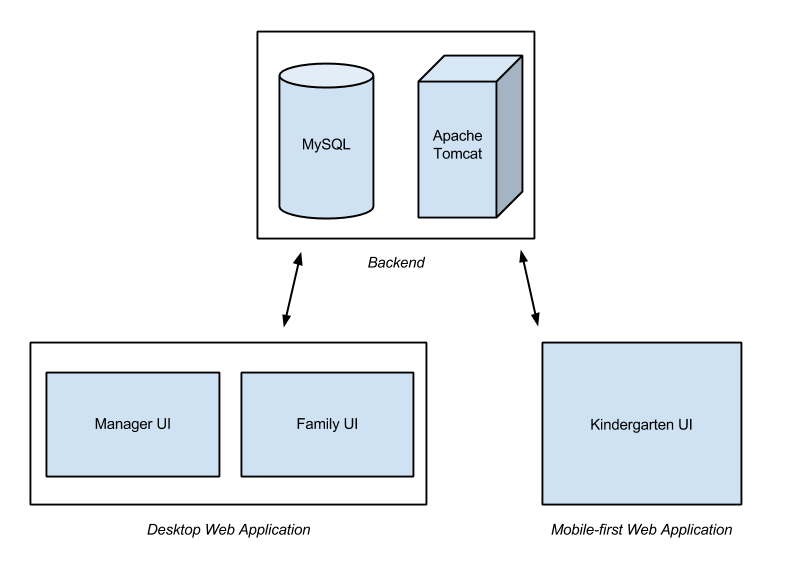
\includegraphics[width=1\textwidth]{assets/architecture.png}
\end{center}
\caption{The high-level architechture of Päikky}
\label{fig:architecture}
\end{figure}



% ##
\subsection{Backend}

The backend is the web server of Päikky which holds all the master data of the system. It serves the HTML content and other resources (graphical assets, JavaScript files, Cascading Style Sheets) to the other modules of Päikky. The backend also implements a REST API which from the other modules requests and alters the data on the system. The abilities the API offers differs between the type of the user's account, but in practice all of the data can be modified via it. Data is exchanged between the backend and the UI modules of Päikky as a JSON objects.

Currently the backend is operated as a single virtual machine on the Amazon Web Services cloud. The data is stored on a single \textit{MySQL} database. The backend is \textif{multitenant}: single instance serves multiple municipalities and kindergartens. % hox todo tänne sellanen numeroviittaus ja termin selitys alareunaan

<tänne selitys Apachen ja Tomcatin suhteesta Päikyssä? vai onko mitään järkeä?>

%-REST API requista tänne jotain, että mitä hä? Hox linkissä tämä-implementation-research (vai tulisko tää tohon ylempään sectioniin?)

<TODO tarvisko jotain lisää kertoa vielä bäkkäristä? mitä? hitusen tynkäkappale just ny>



% ##
\subsection{Kindergarten UI}

Kindergarten UI is the part of Päikky which is used daily by the kindergarten nurses. From the Kindergarten UI nurses can also see elaborate information about the children, including allergies and persons who are allowed to pick them up, have parents allowed the children to be photographed. Nurses can also easily see the contact information for each child. Updating this information is also possible. %They can also monitor the overall presence of persons in the kindergarten, including both children and other nurses.

On Kindergarten UI the key activity for nurses is to log in children (and the other nurses) when they arrive at the kindergarten and log them out when a child or nurse leaves. This activity is repeated tens of times per day. To do this conveniently nurses are equipped with \textit{Android} smart phones. The marking of goings and leavings has to be done in order to replicate the presence status from the real world to the Päikky system. Since monitoring attendance and in the future creating bills for provided daycare is based on the presence data generated by logging the personnel in and out, it is crucial that this activity can be achieved successfully under any kind of condition. Doing this activity should also be as effortless and simple as possible for the nurses so that it would get done at the exact moment when the actual event happens on the kindergarten. 

The simplicity requirement goes for every other aspect of the system: the Päikky users' demography is a very mixed crowd. The kindergarten nurses' age can be anything from 18 to 65. Because of the age variation also the ability and the starting level to use a digital service via smartphone varies a lot. Taking the easiness of usage is also one of the key principles behind Päikky's user interface and interaction design. It is also one of the unique selling points of the company behind Päikky, the \textit{MukavaIT}: "using IT systems shouldn't be hard or unpleasant" [todo viite mukavait.fi].

Based on the plans done by parents on the \textit{Family UI}, nurses can see how many and who of the children they are expecting to appear for each day. If the parents have to change the already existing plans with short notice, automated message is sent to the nurses stating the change, and the plans visible for the child relating the case gets updated in real time. Nurses can also see the exact amount of children and nurses present at the kindergarten for any given time.

As stated above, the attendance of nurses can also be tracked with the Kindergarten UI. With the \textit{Manager UI} it is also possible to plan shifts for the nurses. Combined with the planned attendance data of children done by the parents, this makes Päikky a powerful tool for organizing the kindergarten's daily schedule and ensuring that there are always enough nurses present to take care on the children. This is important since required nurses/children ratio is dictated by law in Finland. % todo tarttisko tähän lakiviitteen?

From technical point of view looking the Kindergarten UI is a single-page web application (explained on the <chapter two> [todo hox viittaus wadap]) created to be used primarily with mobile devices. The libraries the application consists of are: % todo hox tarvitaanko viitettä tohon samsungii? todo tänne semmonen alaviite myös vai?

\begin{enumerate}
	\item \textit{Backbone}\footnote{http://backbonejs.org/}, \textit{Model-View-Template} –framework providing the – wait for it – backbone for the application,
	\item \textit{Marionette}\footnote{http://marionettejs.com/}, library of common design and implementation patterns for Backbone,
	\item \textit{RequireJS}\footnote{http://requirejs.org/}, module loader and dependency manager,
	\item \textit{Underscore}\footnote{http://underscorejs.org/}, functional programming inspired library for utility functions,
	\item \textit{jQuery}\footnote{http://jquery.com/}, utility library for DOM manipulation,
	\item \textit{Moment}\footnote{http://momentjs.com/}, time and timezone handling library. 
\end{enumerate}


The method of data synchronizing between Kindergarten UI clients and the backend is \textit{polling}. Each client sends checksums of it's attendance data to the backend on a regular interval, and if the backend calculates different checksum for the data requested, new data is returned to the clients. This means that if child is logged in to kindergarten with device A, it can take as long as the configured interval for the device B to receive that information. The current interval is 45 seconds. Before the interval was only 20 seconds, but as the user amount increased the current infrastructure which Päikky is run on couldn't handle the amount of requests invoked by that interval. 

The devices and browsers targeted during the development process and which  were delivered to the kindergartens by the client organization were \textit{Samsung Ace 3 Style}'s and the latest stable version of the \textit{Chrome} browser. The devices uses mobile broadband connection as their access method in reaching the Internet. Usually each of the kindergarten's care groups have at least one dedicated device at their disposal. Large groups might have two devices. 

The usual – and most of the time the only – usage environment for Kindergarten UI are the kindergartens around Finland which are using Päikky. The application is used in both outside and inside. Kindergartens can be located practically anywhere, and the mobile reception can vary a lot between different kindergartens. In some locations the coverage and experienced connection quality can be at par with physical broadbands, but the locations with the worst reception are very challenging from the connection speed and latency point of view looking. It is not unusual for the kindergarten to be located on a remote location where getting 3G connection is more of an exception than standard behaviour. % no pitäsköhä tälle olla joku viite:-D


% ##
\subsection{Presence Model}

% -> Presence type/state (kumpi?!), Presence state transfer tms, check implementaation viimeinen kappale

As the primary functionality for Päikky is the monitoring and planning of the attendance of the people on the kindergarten, one of the most essential data models is also the one implementing this feature. The backbone for holding and handling this data is Päikky's \textit{presence model}. In brief presence model is an entity which indicates a range of time when person has had a certain status. These entities are persisted by the Päikky backend on the database.

There are different \textit{purposes} for presences: \textit{actual, plan change, plan} and \textit{default plan}. Each presence has always a single purpose. The purposes are similar for both children and for nurses. Each of the purposes exists on their own domain, resulting in a layered construct of presences for each person. The \textit{actual} presences are the most significant, while the \textit{default plan} is the least significant. % TODO viite kuvaan ja kerrosmallin avaus!°!! 

\begin{figure}[t]
\begin{center}
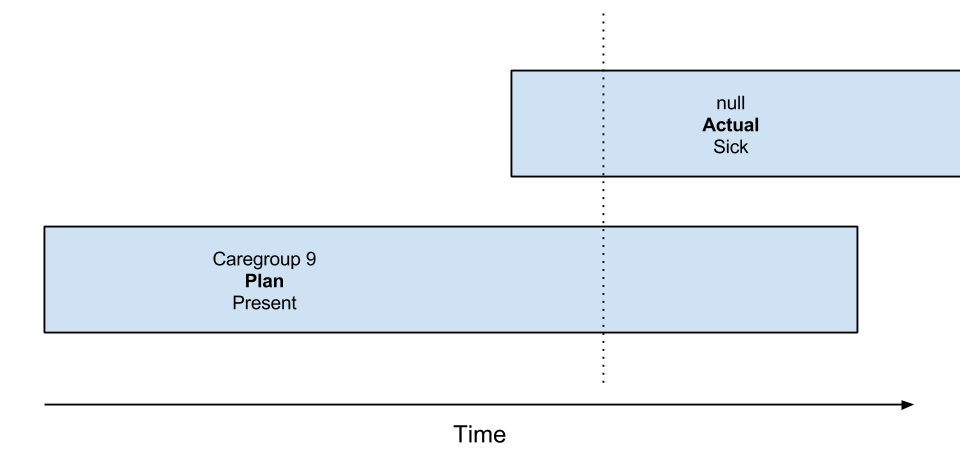
\includegraphics[width=0.8\textwidth]{assets/presencemodel.png}
\end{center}
\caption{The presence model of Päikky.}
\label{fig:presencemodel}
\end{figure}



Each presence also has a single type. The ones used the most are \textit{present, sick} and \textit{day off.} These basic types are the same for children and nurses, but nurses also have a extended set of types indicating specialized reasons for not being at the kindergarten. For example these types includes likes of different cases of sick leaves, trainings and holidays. In this thesis we are concentrating at looking the system primarily from the children's presence markings perspective.

A single presence always belongs to a single person. The presence always has a start time and an end time. There is one special case when presence doesn't need to have an end time (it is then set null on the database): if the purpose for presence is \textit{actual} and that presence is the latest ongoing presence for the person. For example when person is logged in to the daycare on the morning, a new presence entity is created. For this presence start time is set to be the time when he/she arrived to the kindergarten, and end time is left null. This means that this presence is \textit{active} for the current person, indicating ongoing activity. When the person leaves the kindergarten the active presence's end time is set to be the leaving time. If his/hers state is otherwise altered, the active presence is ended and new presence entity with the new type is created. The ending time for the previous presence is the same as the starting time for the new presence. Person's presences with same purpose may never overlap. For single person there can be only one or zero presences per purpose at any given time.



% ###
\subsection{Presence Status and Presence State Machine}

Based on the presence entities of an individual person a \textit{presence status} for they can be determined on any time point. For example if person has a planned presence for the day but they has not arrived at the kindergarten yet, the status would be transcribed as "not yet present" indicating that this person will be present later on today. Mutually if the person has been today at the kindergarten but has already left, their status would be "left for today". The status mechanism is implemented for providing more information about the current attendance status for the kindergarten personnel, in contrary to what simple boolean "present / away" statuses would implicate.

Within presences sharing the same presence purpose, there is a set of rules of allowed state transitions. These rules can be visualized as a \textit{finite-state machine} that shows the possible transitions from different status into another. 

% https://docs.google.com/drawings/d/17hQD7BYT4MUqfRaWlX0ykesfond-cTlAmOQ9Zn9LFQk/edit
\begin{figure}[t]
\begin{center}
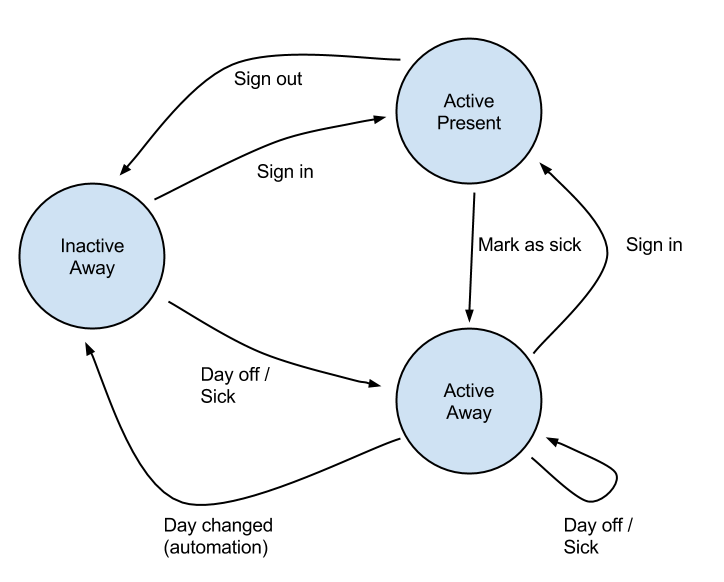
\includegraphics[width=0.8\textwidth]{assets/statemachine.png}
\end{center}
\caption{Presence State Machine. For visualizing purposes this state machine is a simplified version from the one actually implemented on Päikky}
\label{fig:statemachine}
\end{figure}

The figure~\ref{fig:statemachine} describes a simplified version of Päikky's state machine. In this finite-state machine each state indicates two things: is there an active ongoing presence entity for the individual person which has "actual" as the presence purpose ("Inactive~/~Active" on the visualization), and if the current state means that the person is physically present at the kindergarten or not ("Present~/~Away").

Based on the allowed state transitions different kind of buttons for altering the presence state are shown on the person's profile UI. For the most straightforward example if the person is already present on the kindergarten, only a \textit{sign out} button is shown. Since signing in a person already present on the kindergarten is prohibited by the presence state machine, the button \textit{sign in} button is therefore also hidden from the UI. This can be seen on the figure~\ref{fig:child-profile}. 


\begin{figure}[t]
\begin{center}
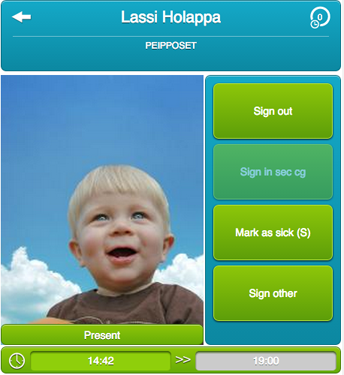
\includegraphics[width=0.5\textwidth]{assets/child-profile.png}
\end{center}
\caption{Screen capture from a child's profile on the Kindergarten UI}
\label{fig:child-profile}
\end{figure}








%% -------------------------------
\section{Emerged Need for Offline Support}
% tänne() taustoja budurajotteista, käytettävissä olevista henkilömääristä jne 
% -> miksi tehtiin niinkin paljon kompromisseja kuin tehtiin (budu, MVP-lähestyminen)
% -> Pete-haastiksesta (mukavait tj) kamaa
% -> HOX PÄIVÄMÄÄRÄT SELVITETTÄVÄ; ainakin milloin offline-moodin rollout tuotantoon?

% Tänne jotain tavaraa (mahdollisesta) Päikky-toimitusjohtajan haastattelusta (jota ei siis vielä ole tehty?). Ehkä jos jotain löytyy kommunikaatiosta/kehitysdokumenteista niin se myös?

% Kannattaisiko tänne kaivaa versionhallinnasta dataa offlinemoodista, tyyliin millä aikavälillä se kehitettiin, paljonko arvioitu rivien määrä, etc? Vai voisko tämä knoppitieto olla jossain muualla? Tai ylipäätään missään?






% ##
% \subsection{Before and after Offline-mode}
% tämä kappale on toistaiseksi hyllytetty. jos tästä 
%-> Softan käytöstä ennen/jälkeen offline-modea (onkohan tää ny turhaa asiaa ylipäätään?)









%% ---------------------------------------
%% Research Methods 
\chapter{Research Methods}
% Implementaatiosta sen verran että tutkimusmetodina on implementoida teknologiaa ja tutkia kuinka se soveltuu arkipäivän käyttöön. Voisi myös miettiä lähestymistä että sulla on ollut kaksi eri tilannetta 1. softa ilman offline"palikkaa/featurea" ja 2. offline palikan kanssa. Tutkit että kuinka offlinepalikka vaikutti sovelluksen käyttökokemukseen.

%% ------------------------------------------
\section{Design Research}
Tähän jotain... tiedettä... jostain...

"Konstruktiivinen tutkimus"
% Pyry-viitehox: Pertti Järvinen ja Annikki Järvinen - Tutkimustyön Metodeista

Piirainen-Gonzalez kirja Dropboxista


%% ------------------------------------------
\section{Data Collection with Semi-Structured Interviews}
% MikkoKoski-dipasta saa hyvää mallia tähän

"Validating Offline mode User Experience with User Interviews"

Avattu, keneltä on kysytty (päiväkodin tädit) mitä (Päikky-järjestelmän käyttöä ja offline-moodin käsittämisestä juttua) ja miksi (pyritään ymmärtämään onko offline-mode vastaus todelliseen käyttäjien ongelmaan). Datan keräysmetodina puolistrukturoitu käyttäjähaastattelu.

\subsection{Finding Interviewees}
Ketä haastateltiin, millä perusteilla valittiin


\subsection{Preparing Interviews}
Miten haastattelurunko tehtiin


\subsection{Conducting Interviews}
Miten haastattelu toteutettiin


\subsection{Analyzing Interviews}
Miten analysointi tehtiin

% datan keräysmetodina käyttäjä/asiakashaastattelut (muuta?, kehitysdokumentit?)

  

 
%% ---------------------------------------
%% Implementation

\chapter{Implementation}
This chapter coverages what was done to the Päikky system in order to get it working also during the Internet connection shortages, and how that was done. 

This chapter is concerned with the facts of what the offline mode consists of and how it was implemented. Reasoning for the decisions made are also explained. Analyzing the consequences of those decisions are done later on the evaluation chapter.

%% --------------
\section{The goal for the Offline support}
% tämä case päikky -lukuun?

% Mitä Offline-modella TAI SIIS SUPPORTILLA pyrittiin saavuttamaan?
<META: Pitäisikö yleisemminkin erottaa offline TUKI ja kindergarten-UI:n offline MOODI? Tulisiko tämän tavaran olla jossain muualla kappaleessa kuin täällä?>

The primary goal for the offline support on Päikky was to enable the most critical tasks for kindergarten nurses on all situations [?petehaastattelu?] on the Kindergarten UI (the mobile friendly version of the Päikky system). 

Päikky's main and the most important feature is the ability to track the attendance of the kindergarten's children on real time. In order to achieve that, nurses must be able to mark the children's coming and going without getting interrupted by the limitations of the application. In order to offer offline support on the Kindergarten UI, a new feature called \textit{Offline mode} was implemented. Offline mode aims in removing the Internet connection quality related limitations on the nurses' key activity. Nurses should be able to use the children logging feature on Päikky under any kind of Internet condition. If the Internet connection is nonexistent, the application should record user's actions and save them to the server once the Internet connection is achieved again.

Secondary goal for the offline support were to allow as seamless usage as possible of the Päikky on kindergartens where Internet connection is weak. Nurses should be able to see the information from Päikky even if there is no Internet connection at the time. Information should be served based on the best-effort delivery: application should show all the information it has at the time to the user while trying to fetch the most latest version of the information.

Other parts of Päikky – the \textit{Manager UI} and the \textit{Family UI} were left out of the offline support.

The ultimate vision - yet to be reached - for the offline support is that it would abstract the Internet connection quality completely away from the user's consideration. Under any connection quality the user should be able to use Päikky normally without any interference. On the current version this is not yet achieved (nor it was scoped to be achieved). % saisko tähän kappaleeseen jonkin viitteen johonkin käytettävyys-diibadaapaan, johonkin käyttäjän "mielenmalleihin" tms eli siis että ultimate goali olisi, ettei käyttäjän tarvitsisi huolehtia tuosta verkon laadusta ollenkaan, jopa niin että käyttäjä ei edes tietäisi ollaanko online- vai offline-moodissa?




%% --------------
\section{State transitions to and from the Offline mode}
% offline ja online -moodin selitykset, termien avaus? erityisesti "online-moodi" (jos online-moodia ei selitetä, niin sitten ainakin pitää muissa kappaleissa puhua jostain muusta kuin online-moodista)

% HOX onko päällekkäisyyttä methods-case -kuvauksen kanssa?
Implementation of the offline support to the Kindergarten UI made it to have two different states related to the Internet connection status. Application is on the already mentioned \textit{Offline mode} when the Internet connection is poor or nonexistent, and on the \textit{Online mode} when the Internet connection is working normally. 

The current mode is implicated to the user clearly: while in Offline mode, the Kindergarten UI's header changes color scheme to greyscale and the title says directly \textit{"You are working on the offline mode"}, localized to the user's language.

While in Online mode the Kindergarten UI works almost identically as it did before the offline support implementation. Major changes are that all the API requests done to the Päikky backend are cached to the Local Storage of the device running the Kindergarten UI. Also the sending of Presence marking changes to the backend are done by a dedicated component. Both of these are primarily refactoring the inner parts of the Kindergarten UI, while using the application the user should not experience any difference to the versions prior from these changes.

When entering the Offline mode the method on how data is fetched changes. Instead of fetching the data user requests from the backend, the Kindergarten UI fall backs to the data cached on the \textit{Local Storage}. This won't guarantee the availability of the up-to-date information to the user, but at least showing the best effort version is possible. Due to the nature of the Päikky's data, in most of the cases this is acceptable (e.g. when looking for children's parents' phone numbers, and other similar data that is not altered on daily basis). Also some of the features on the Kindergarten UI are disabled when the Offline mode comes active. This functionality is described thoroughly on the <Using Local Storage as a Cache> -section [hox-todo].

While the Offline mode is active, the component responsible for sending the Presence marking changes – the \textit{Job Queue} – acts also differently. If there is a recognized issue with the Internet connectivity (which triggers the Offline mode to be activated), Job Queue stops sending the Presence Markings to the backend but instead saves them to the Local Storage. User is notified on this by showing all the time the size of the queue on the top right corner of the Kindergarten UI. When the Internet connection is active again, the Job Queue starts to send the cached Presence Markings to the backend one at a time. This functionality is explained in depth on the <Job Queue> -section [hox-todo]. 





%% --------------
\section{Limited Feature Set on the Offline mode}
% Offline-moden rajoitettu featuresetti - mitä ja miksi

Similar to every other real life software project also in Päikky compromises have been made while balancing between the scope, the available resources and the quality of the end product. In order to create software with good quality under given budget, the scope had to be kept reasonable and some prioritization between features had to be made. This resulted the first version (the one studied by this thesis) to be technically quite simple and even naive on some aspects. Users experience this as a lack or disabling of some features on the offline mode.




%% ###
\subsection{Disabled features}
When the application enters the Offline mode all the features except the critical key functionality are disabled from the user. These include features such as

\begin{enumerate}
    \item sending messages on the application,
    \item editing persons' information,
    \item changing persons' photos,
    \item editing existing presence markings or upcoming presence plans.
\end{enumerate}

These features were left out from the Offline support based on feature importance evaluation done by the customer [?todo-hox petehaastis?]. Since under available budget some features had to excluded from the offline mode, the ones listed above were selected due to the nature of their basic use case.

None of the listed activities are essential for the Päikky's key feature, the real time tracking of kindergarten's personnel attendance. If there is no Internet connection available at the time, each one of these activities can be postponed without sacrificing the integrity of the presence data on the system until the Internet connection is available again.




%% ###
\subsection{Simplified Data Synchronizing}
% synkkaus-yksinkertaistus-juttui
% nonexistent collision check!
% googlewavepaprusta jotain dadaaa tänne?
The nature of the Päikky usage by the nurses allowed the development team to make some simplifications to the implementation of the offline mode. These simplifications included the way how conflicts between concurrent changes are solved. To put it bluntly, they aren't solved in any way.

To understand why this solution was feasible, one has to understand the environment and practices about how Päikky is operated. The usual scenario on the kindergartens where Päikky is used is that each kindergarten group has only one, dedicated device. With minor exceptions all of the presence markings for the care group's personnel are done via the group's dedicated device, which is also the only device for the group to access Päikky. This is also the way how usage of Päikky is instructed by the client organization to the kindergarten personnel. Editing person's presence status from different devices while on offline mode is especially discouraged. With these guidelines the probability for cases where two different devices have made concurrent changes to individual person becomes almost non-existent. [?todo-hox tähän Pete-haastiksesta vahvistus?]

These circumstances allowed the development team to streamline the data synchronization on the Päikky server. On agreement with the client organization, there is no functionality that tries to solve possible merge conflicts on the presence data. If there appears a situation where two devices have concurrently changed the attendance status of a single person - contrary on the instructions given to the users - both of the changes are saved to the database. Fixing the data to reflect the situation happened in the real world is left to the responsibility of the kindergarten personnel.

The decision which passed on the responsibility of the data correctness to users also removed functionality needed on the Päikky backend. Because of this the work done in order to implement the required level of offline support to Päikky was almost entirely done to the Kindergarten UI. The backend required only minimal changes relating this. Read more about the backend changes on <Storing and Receiving Pres....> section. [todo hox mite nää viittaukset]
% backend-offline-tuen olemattomuus myös tässä?

This approach removes the need of offline related functionality on the Päikky server almost completely. By this the development effort was cut significantly: the probability of creating data conflicts has been made minimal with the user instructions, and in the implausible case of a conflict to appear resolving it is left to the responsibility of the user, not by the code base. 

From the server point of view, presence markings done on the offline mode are received and stored exactly same way as are the markings done real time on the online mode. Only thing that differs is the time gap between the presence marking's timestamp and the occasion when the presence marking is received on the server. This is described in detail on the section <Storing and Receiving Presence M...>[todo-hox]. % tämä ehkä muualle?





%% ----------------------------------
\section{Technical Details}
% HOX tää koko setti on lähinnä frontendissä, backendiin ei juurikaan tehty mitään lisätemppuja offline-moodia varten??
The technical details of the implementation covers almost entirely only the Kindergarten UI of the Päikky system. This is due to the allowed boundaries for the development team and the real life limitations of the Päikky system usage. In order to achieve the required level of offline support on the system, almost all of the work could have been done only on the mobile frontend codebase: the Kindergarten UI. In addition to the changes made to the backend, no other modules (\textit{Family UI, Manager UI}) of the system needed changes. However the other modules did not gain any kind of added offline support either.


%% ###
\subsection{HTTP Cache Headers}
% maininta, että tämä olisi ollut hyvä tehdä myös ilman offline-tuen tekemistä
% TODO:
% - pitäisikö tänne vielä erotella API-pyynnöt omiksi jutuikseen? Nehän tulee tosin Tomcatilta, käpisteleekö Apache sinne headereita ollenkaan? 
% -> API-pyynnön response headerit:
% Access-Control-Allow-Origin:*
% Connection:Keep-Alive
% Content-Type:application/json;charset=UTF-8
% Date:Mon, 24 Nov 2014 12:45:59 GMT
% Keep-Alive:timeout=5, max=99
% Server:Apache-Coyote/1.1
% Transfer-Encoding:chunked

% mahdollisia viitteitä:
% - http://tools.ietf.org/html/rfc2965 (????)
% - http://www.w3.org/Protocols/rfc2616/rfc2616-sec14.html#sec14.9 !

Starting point for the offline support implementation was to take as much advantage as possible from the techniques already in use on the Päikky system's implementation. First task for the development team was to ensure that the cache related features of the HTTP protocol were utilized thoroughly.

Previously there were issues reported by the users after production environment updates that the new features announced weren't visible on their devices. This was the result of poor and some part nonexistent cache header usage. The cache headers prior the change instructed the browser to save the \textit{index.html} document – the starting point of the Kindergarten UI web application – and all the JavaScript files for 24 hours on the file system of the device. If those files were requested within that 24 hours, the cached versions were used. This created a huge lag on the rollout of the latest version to the end users' devices, which caused work for the development team since both the old and the new version of the frontend client had to be supported on the backend.
% HOX tsekkaa tästä kappaleesta toi vanhan cachetusajan pituus, emmä muista, tuo 24h on vejetty stetsonista :----D 

The "release lag" was addressed by altering the HTTP 1.1 headers related to caching, which are returned by the Päikky backend's Apache web server to the browser. The first solution was to disable cache entirely, forcing the browser to fetch the data again each time from the backend while browsing. This was achieved via the following headers:
% päikky main.js -nykyrequsta:
% [TODO-HOX koodityylit, ja joku caption tälle, miten?]
\begin{lstlisting}
    Cache-Control:max-age=0, no-cache, no-store, must-revalidate
    Pragma:no-cache
    Date:Mon, 24 Nov 2014 08:36:04 GMT
    Expires:Wed, 11 Jan 1984 05:00:00 GMT
\end{lstlisting}
%\lstinputlisting[caption=Päikky HTTP Cache Headers] [hox-todo, nämä aiheutti jonkun latex-oksennuksen, tarkista myöhemmin että how do i shoot web, sama alemmassa koodilistauksessa]
\noindent The goal with these headers is that the browser saves intentionally none of the content it receives. Achieving this is done by several mechanisms to cover the most of the browsers in use. From the HTTP 1.1 protocol view of point some of the instructions overlap each other (e.g. Pragma:no-cache and Cache-Control:no-cache) while some are there to address the HTTP 1.0 protocol (using Expire-date from the past). [Fielding, et al]

Using these headers solved the release lag problem and streamlined the production deploy process, but otherwise did little to actually help the development team to get closer to the offline support on the system. Actually these changes made the Kindergarten UI to be more reliable on Internet connection, since browsers were instructed not to save any data fetched from the Päikky backend. This also increased the average loads of the backend.

To take advantage of the HTTP Cache Headers from the offline support perspective, different cache rules were made for the most bandwidth-greedy assets: the images. On the Apache web server following headers were set to be sent on response to each request that were made for images, no matter if they were graphical assets to the web application (icons etc) or profile pictures of children and nurses:

% päikky kuva-nykyrequsta:
% (86400s == 24h)
\begin{lstlisting}
    Cache-Control:max-age=86400
    Content-Type:image/jpeg
    Date:Mon, 24 Nov 2014 12:41:01 GMT
    Expires:Tue, 25 Nov 2014 12:41:01 GMT
\end{lstlisting}
%\lstinputlisting[caption=Päikky HTTP Cache Headers for images]
\noindent These headers allows the browser to cache the image for 24 hours. For person profile pictures there won't be any lag on updates when the image changes. Every picture gets a generated unique file name on the upload, so from the browser's point of view they are totally new pictures instead of new version of the old picture. The cache validness duration can therefore be decided based only on how fast the update cycle on the graphical assets of the needs to be. If generating unique names for the graphical assets would be done on the production version build phase, this cache duration could be increased to e.g. one year and only side effect would be increased cache sizes on the clients' browsers.

Addressing the HTTP cache header related problems were not directly coupled to the enabling of the offline mode, but fixing them would have benefit the Päikky system even if the offline support would not have been on the product's road map.







%% ###
\subsection{Application Cache}
% Tänne kappaleeseen saa tarvittaessa paljon lisää kamaa tosta "appcache is a douchebag" -artikkelista, sudenkuoppia jne
% responsiiviset erilaiset kuvat -issuesta maininta?

% UHHHH TIMANTTISTA LÄHDETTÄ TÄÄLLÄ http://dl.acm.org/citation.cfm?id=2307649 katso erityisesti kohta "[3]" !!! [Qian et al.]

HTML 5 specification adds a new tool aiding the creation of offline supported web applications: the Application Cache. The specification was designed to allow creating of web applications that would work (after caching) without Internet connection, but it is also useful in decreasing load and start up times in a normal, Internet-aided usage. 

Application cache is initialized by creating a Cache Manifest file for each HTML document. In Single-Page Applications, which Päikky also is, this is achieved easily since as the name implies there is only a single HTTP document for the whole web application that needs to be loaded [HTML5 spec].  Whereas HTTP headers regarding cache rules addresses the problem with generic information about the expiry date of the fetched resources, cache manifest states more elaborate instructions for situations where Internet connection is unavailable. [Qian et al.]

\begin{lstlisting}
CACHE:
js/configurations/local.js
js/main-b13f3e6.js
img/icon_delete.png
img/paikky_logo.png
css/client.css

NETWORK:
*
\end{lstlisting} % Snippet from the Päikky Kindergarten UI's Application Cache Manifest

On the listing <x> [todo-hox viittaus tuohon päikky cache manifestiin] we can see a shortened version of the Cache Manifest of Päikky's \textit{index.html} and how it describes the nature of the resources to the browser. On the complete version of the Päikky's manifest each of the known resources for the application is listed under the "CACHE:" -notation, which means that these resources should be cached by the browser. After that everything else is whitelisted with the "*" wild card to be downloaded from the network. The whitelisting of the rest of the possible resources is important, since when working with the Cache Manifest browser tries to do exactly as stated on the manifest. This means that if that wild card network rule would be removed, the browser wouldn't be able to fetch the resources not listed on explicitly stated on the manifest. [Lawson and Sharp s. 212] % hox tuosta serverin lataustavasta ei ole mainintaa tuossa kirjassa (ainakaan en löytänyt vielä), vaan se on peräisin appcache-douchebag-artikkelista

% REDUNDANTTIA TAVARAA 
%The Application Cache also differs from the HTTP caching by not defining expiration dates for individual resource, but instead all of the cached resources are re-downloaded every time when the manifest updates. If the expiration date set to the resource concurs before updating of the manifest file, the resource is re-downloaded. Also when using the % TODO-HOX pitääkö tämä varmasti paikkaansa?

When using the Cache Manifest it must be noted that even when the user is online, the files are served from the Application Cache. Developers must also notice that updating the resources listed on the Cache Manifest is not enough. Browser doesn't re-download them if the manifest itself is not updated (or if the cache expiry date set by the HTTP headers for individual resource doesn't expire) When visiting a site with a cache manifest again, the browser renders the first version of the site with resources stored on the Application Cache, and only after that connects to Internet for checking possible updates to the content. [Archibald, J]

Due to the nature of the cache manifest (has to be updated on every web application update, has to handle each of the resources somehow) it is highly recommended that the creation of the manifest file is automated as a part of the build process of the web application. On Päikky's Kindergarten UI this is done with the \textit{grunt-manifest}-tool every time a new production version is created. For the development environments a different, static cache manifest is used, which tells the browser not to use the application cache at all.

It is also possible to insert a fallback version for the resources on the Cache Manifest that are used if the network connection is unavailable. In practice the manifest can state alternate version for resources to be used, if there is no network connectivity. This can be useful in some browser heavy applications that use minimal amount of data from the Internet, e.g. applications like \textit{Google Spreadsheet} [Using the application cache]. However this was not seen useful on the implementation of Päikky's offline support and therefore was not used. % hox-todo numeroviitejuttu tohon google spreadsheettiin

As was the case with the HTTP Cache Headers, the Cache Manifest would also have benefit Päikky even if the offline support wouldn't have been implemented to the system.

% pitäisikö täällä mainita jotain tästä http://alistapart.com/article/application-cache-is-a-douchebag ?






%% ###
\subsection{Monitoring Connection Quality}
Identifying connection issues is a key activity regarding the Offline mode. When a connection issue is noticed, the Kindergarten UI fall backs from the Online mode to the Offline mode. While on the Offline mode, the application must monitor the health of the connection to determine when it is safe to use the network connection again.

On Päikky the connection quality is monitored via errors on \textit{Ajax requests} [ajaxError], triggered by the \textit{jQuery}-library. As described on the Backend-chapter, the Kindergarten UI communicates to the backend via REST API requests for different kind of resources. There is an application level error handler for cases when one of these requests should fail:
\begin{lstlisting}
    // Function for identifying network related Ajax errors
    var isOfflineTriggerError = function(thrownError) {
        return _.contains([
            'timeout', // "JavaScript-level" timeout
            ''         // "network-level" errors - all of them
        ], thrownError);
    };

    // Error handler for Ajax errors
    $(document).on("ajaxError",
        function (e, jqXHR, ajaxSettings, thrownError) {
        // List of exceptions that triggers offline-mode
        if (networkStatus.isOfflineTriggerError(thrownError)) {
            vent.trigger('offline');
        }
    });
\end{lstlisting}
\noindent
In practice Kindergarten UI triggers Offline mode on two different kind of errors: if there is a error coming from the JavaScript-level (usually meaning that no response for request was received within the configured time period) or if there was an error on the network level (connectivity was nonexistent). In these cases an \textit{offline-event} is triggered via the \textit{vent}, the event bus of the application.

Modern browsers implements also the \textit{navigator.onLine}-property which indicates the network status as a boolean value. Despite the promising specification this can't be the only way of checking the network connectivity, since the behaviour is heavily dependent on the browser. For example in \textit{Chrome} and \textit{Safari} having only a connectivity to local area network will result the onLine-property being true. [window.navigator.onLine]

After the application has entered the Offline mode, it halts all the Ajax requests except a specified \textit{ping}-request to the backend which is used to determine the health of the connection. If the ping should fail, another ping request is scheduled. There is a maximum time interval configured on the application in which the response must be received. Only after a successful ping request within the allowed time range the pinging is stopped and the Online mode is activated again.

% tänne vois kirjottaa pingin yhteydessä tapahtuvasta kellosynkkauksesta, jos tarvii lisätekstiä? muuten ei ehkä hirmu oleellinen network statuksen suhteen
% iteasiassa onko sittenkin, sitähän käytetään noiden presence markingien teon yhteydessä




%% ###
\subsection{Using Local Storage as a Cache}
% Local storagen perusteet
% REST-API-pyyntöjen cachettamisesta local storageen juttua
% hox [Casario et al]

The new HTML5 standard adds also another important tool for the Päikky's offline support to take benefit from: the \textit{Local Storage}. It is an origin specific storage which saves its contents to the user's file system and persists them between sessions. While being only a simple key-value -storage it is not the most sophisticated solution for client-side storage mechanisms there is available on the modern web development toolbox, but for simple use cases like the Kindergarten UI it's simplicity is a decisive advantage.

While being on the Online mode, every request made by Kindergarten UI to the backend's API is stored to the Local Storage. The request's URL is used as the key for the entry, and the response of request is saved as a value for that key. At the current version of the application there are no optimization mechanisms implemented with the Local Storage content. When Internet connection is available the saved responses are ignored. On each request the possibly already existing responses are overwritten.

After the Offline mode is activated the Kindergarten UI continues to make API requests based on user's actions. But instead of making them to the backend's API, the \textit{Backbone}-library – which is responsible for data fetching and synchronizing on the application – forwards the requests to the Local Storage API, where cached versions of the once fetched requests can be found. This allows the user to navigate within the application and see the latest version he/she has fetched from the backend. If the user navigates to a view not visited before, view without the actual content is rendered. 

Due to the limited feature set of the Offline mode (as described on the section <x> [todo-hox viite tuonne yläkappaleeseen tähän]) there is no need for checking dirty cache entries [Laplante s. 138], since user can not alter the cached data while having no Internet connectivity. Only after the Online mode is activated the editing of the data is made possible, and then the contents of the cache is ignored. Exception to this are the \textit{Presence Markings}, whose are explained in more detail on the following section.


% miksi tämä tehdään local storagella eikä esm cache manifestilla? -> selitä(?

% HOX tietoturvaongelmat tämän suhteen (ei tässä keississä mutta yleisesti), problematiikka tämän tiedon kryptaamisesta -> ei mahdollista





%% ###
\subsection{Job Queue: Promise-based Presence Marking queue}
% Kuuluiskohan tuo promise-konseptiosa related researchiin ennemmin?
% hox presence markingien LUONTI vs. olemassaolevien muokkaus?

% https://github.com/futurice/mukavait-paivahoito-kindergarten-ui/blob/development/src/js/JobQueue.js

The key activity for nurses recognized before on this thesis is the altering of the kindergarten's personnel presence data. This activity must be available for user no matter what the Internet connection status is. Allowing this activity was also the primary goal for the offline support to have. With the resource limitations the development process had it was therefore apposite to create a dedicated mechanism for syncing specifically this data and disabling other data altering features while the Offline mode is active. % todo-hox oliko näin?:-D

On the Kindergarten UI this is enabled by a component called the \textit{Job Queue.} Job Queue is an array of jQuery's \textit{Promise} objects. Each of the objects on the array represents single Presence Marking to be saved to the backend. Every time user creates a new Presence Marking it is added to the queue, no matter if there if an Internet connection problem is recognized or not.

% HUOM .promise jquery specistä:
% The deferred.promise() method allows an asynchronous function to prevent other code from interfering with the progress or status of its internal request. The Promise exposes only the Deferred methods needed to attach additional handlers or determine the state (then, done, fail, always, pipe, progress, and state), but not ones that change the state (resolve, reject, notify, resolveWith, rejectWith, and notifyWith).

The concept of "promise" was first time introduced in 1976 by Friedman and Wise [Friedman and Wise]. It is used to describe an object which value is yet to be resolved, being a temporary placeholder and a \textit{promise} for the to-be value. In asynchronous languages such as JavaScript this is highly useful since for example when fetching data the developer can't trust that the results are available immediately after the request. Promise makes sure that altering the state or the progress of its internal request is not possible from outside. This makes it an ideal capsule to wrap the Ajax requests with. [deferred.promise] % todo-hox miten tässä viittaaminen tohon antiicciseen teokseen? entä onko tossa viimesessä lauseessa mitään järkeä? :--D

%%%%%%
KUVA-TODO tänne joku hieno kaavio tosta promisejonosta?
%%%%%%

When user creates a new Presence Marking on the Kindergarten UI (e.g. logs child in to the kindergarten when he/she arrives), a new Promise is created which includes Ajax request to the backend. Request's payload is the new Presence Marking. That Promise is then added to the Job Queue. 

While the Online mode is active, Job Queue constantly looks for the oldest job on the queue and tries to execute it. Executing it means activating the Ajax request inside the Promise. After the request is successfully sent to the backend and a response is received, the promise marks itself as \textit{solved} and that job is then removed from the queue. This process is repeated within a configured interval as long as the application is active on user's browser. If an ongoing request fails due to a network error, the application fall backs to the Offline mode, and the Job Queue execution halts until Internet connectivity is gained again. It is possible for the request also to fail due a e.g. mismatched parameters, which causes the job being removed from the queue.

The state of the queue is persisted on the Local Storage to address the case if the user shuts down the application before the whole queue is sent to the server. Therefore every time the application starts the queue is initialized from the contents stored locally on the user's browser. However also this solution outsources some of the responsibility to the user: in order to have up-to-date information about the attendance status every nurse must ensure that the queue is empty when their shift ends.  % HOX onko näin oikeasti? HOX TODO pitäisikö viimeisen lauseen juttu siirtää evaluation -kappaleeseen?




%% ###
\subsection{Storing and Receiving Presence Markings on the Backend}
% "Storing and Receiving Presence Markings on the Backend"
% - ainoa offlineen liittyvä muutos mikä toteutettiin bäkkäriin
% - presenceille timestamp, milloin ne on tehty -> voi (ja on) eri kuin mitä vastaanottotimestamp on
% -> yliyksinkertaistaen käytännössä kaikista merkinnöistä tuli "offlinessä-tehtyjä" verrattuna aikaisempaan, missä merkintöihin otettiin timestampit serverille saapumisajan mukaan
% - Tänne jotain juttua kellosynkasta pingauksen yhteydessä? Vai pitäisikö siitä taruilla ton network-laatutunnistuksen yhteydessä?

Due to the simplicity of the offline support required for Päikky, most of the code related work was done on the Kindergarten UI only. Only offline supported feature which needed modifications to the backend was the ability for the user to create Presence Markings without active Internet connection at the time. This required some changes to be done on the mechanisms which receives and stores the Presence Markings coming from the Kindergarten UI. 

Before the offline support Kindergarten UI did not send timestamps of the created Presence Markings to the backend. Timestamps were created on the backend at the time when the requests from the Kindergarten UI were received. 

To allow the postponed sending of the Presence Markings created in the past, the responsibility of creating the timestamps for the markings had to be moved from the backend to the Kindergarten UI.

<TODO tänne selitystä kellosynkasta>




%% ###
\subsection{Duplicating the Presence State Machine}

% (tarviikohan tämän välttämättä olla oma otsikkonsa?)
Before the offline support the backend also validated the state transfer for the Kindergarten UI. If the new Presence type requested by the application was invalid, the backend would have returned a legal state, which the Kindergarten UI would have applied to the current person. From the user experience point of view this could be seen as a slight lag on the changing of the person's state when the new Presence marking was created. Kindergarten UI at time would not have known what the new state would be and therefore was forced to wait for the backend's response. 

%Since there is always a restricted amount of legal presence state transfers, allowing the Kindergarten UI to set the timestamps for the Presence Markings required it to know about the allowed state transitions from a presence status into another. 

In order to enable the Kindergarten UI to know the allowed possible state transfers and to determine the new Presence state. This resulted as a need for duplicating the Presence State Machine (described on the <chapter three> [todo hox viittaus]) from the backend to the Kindergarten UI. Duplicating it created some redundancy to the backend and Kindergarten UI codebases. Having the Presence state machine on both components of Päikky was inevitable, since as the keeper of the master data, removing the state validating from the backend would be shortsighted. Requests made to the API can be tampered with, and the actual payload has to be always validated by the backend. However having the same validation in two places creates a challenge for the developers: both have to be kept in sync in order for the system to operate properly. 

On the bright side the lag on the user interface with the Presence state transfer got minimized with the added functionality, since new state could be determined on the browser without having to wait for the backend interaction's result.





















 

%% ---------------------------------------
%% Evaluation: teh Results
\chapter{Evaluation}

This section goes through the results got from the interviews. Solutions and compromises done on the technical side are also evaluated critically.


%% -------------------------------
\section{User Interviews}
% caption=User Interview Results?
% Validointi haastattelujen kautta, mitä mieltä offlinen toimivuudesta
% HOX mikkokokski-dippaan, täällä on enemmän ollut selitetty noita haastateltavien tyyppien valintaprosessista yms. Tässä mun versiossa kaikki tarpeellinen on imo kerrottu jo methodseissa, joten ei ehkä niin tärkeä tässä?

% <meta todo hox: onko jako tämän ja methods -kappaleen sisältöjen välillä hyvä? pitäisikö veivata kamaa eestaas joltain kohdin?>

This section covers the analyzed results from the interviews. Main goal is to validate the prediction that the user experience of the offline mode is supporting the actual use cases on the kindergartens. Full transcriptions of the interviews are not available.

All of the users interviewed were full-time kindergarten nurses. Average age for the interviewees was 36,5 years. Youngest interviewee was 31 years old and the oldest was 52 years old. Both kindergartens where interviews were executed were opened fairly recent making the average length of employment only about 1,5 years (exact length of the employment periods were not questioned). Nevertheless there were lots of experience from the day care sector within the interviewees; the oldest interviewee had started their career on this field of operation in 1997.

Interviewees were asked about what kind of phone they own, and how they would describe their skills on taking advantage from the phone. This aimed at charting the readiness and the base level of the user in using a digital service via smartphone. 

Only one of the interviewees didn't have a phone that couldn't be described as a smartphone. They were also the only one who directly stated that their skills on using modern devices were fairly low. Other interviewees had smartphones, but only one had a smartphone sharing the same operating system used by Päikky. That correspondent was also the only one who described themselves as an advanced user of a smartphone. Other two stated that they can achieve basic functionality without much hesitation, but everything beyond that would be a challenge from some magnitude. 

The mobile network coverage varied a lot between the kindergartens. The other was said to  have fairly good reception on most of the places, while having couple of dead spots. On the other kindergarten the reception was reported to be very bad, and this was also noticed by the interviewer when arriving on the premises. 

The interviewees are not referred by their real name or the kindergarten they work on. Referring them is done by a randomly generated <todo hox footnote-viite random.org> number from a range from two to ten. The linking between interviewees or kindergartens and the generated numbers is not available.



% ###
\subsection{General Feedback from the Päikky Usage}

In general the interviewees stated that they are satisfied with Päikky, and that it makes a lot of the daily activities easier. For example looking for children's parents' phone numbers from Päikky is a really straightforward and simple task in contrast to the old way of finding them from paper archives. 

Nevertheless neither of the kindergartens did use Päikky as the only method of recording children attendance on the day care. Both kindergartens created markings also in writing to the \textit{care group diary}. Goings and leavings didn't get marked to the diary as precisely as they get to Päikky though; no time markings were written into it. The diary logs could be seen more of an coexistence of a legacy system than a direct backup method. The diaries have existed long before the implementation of Päikky, since they were the method for tracking attendance prior it. 

Non-surprising result from the interviews was that each of the interviewees stated the logging of children in and out as the activity they do the most with Päikky. This was said to be done tens of times per day.

At the start of the Päikky usage parents asked quite often instructions from the nurses. Interviewees stated that this stopped shortly thereafter. Mostly this was caused by the nurses instructions which told the parents to contact the client organization's help desk in case of issues. In day-to-day interaction with parents the interviewees said that Päikky didn't usually come up as an topic, unless there were some issues with it. Usually the issue was parents who forgot to add care plans for their children.

Interviewees from the other kindergarten said that they have successfully moved all the communication between the homes and the kindergarten to be done via Päikky. The other kindergarten also used Päikky as their primary communication channel, but on addition to that they had standard procedure on communicating via paper which was used on some occasions.

All the interviewees told that within the nurses Päikky is a daily topic. Interviewees number 9, 2 and 5 stated that sometimes they vent their frustration with blaming Päikky out loud to fellow colleagues. More often talks relating to Päikky were regarded syncing with colleagues that did they correct some noticed inaccuracy on the attendance data or something else relating to correction of the markings.

Interviewee number two said that in their care group Kindergarten UI was often used on a desktop computer. Also the standard way of using it via smartphone was in use. The desktop computer was mostly in use due the easiness of the usage, and the central location of the said computer. 

Interviewee number eight stated that if there appears any issue with Päikky, they usually tries to find someone else to solve it. Other interviewees couldn't remember an issue with Päikky that they couldn't handle. Only exception for this was the case on the other kindergarten's devices, which would seemingly load Päikky everlastingly on the start. On situations like that the loader icon wouldn't disappear after user started Kindergarten UI from the home menu, making the using of the application impossible. This was fixed on an update to the system later on.


% ###
\subsection{User Experience on the Offline Mode Implementation}

All the interviewees stated that they would always notice if the application goes to the offline mode. The offline mode header was said to be too eye-catching to be missed.

When the application entered offline mode, common model of operation was just to wait for the connectivity to be reached again and keep on using the application on the offline mode as best as they can. Interviewees were asked if they had a habit of going to a specific place in order to achieve better reception, but this was said to be impossible since the nurses found themselves usually in a situation where they where the currently only supervisor for the children, and therefore they were unable to move. One interviewee said that they sometime try to move the device higher while trying to get a better reception.

Interviewees from the first kindergarten reported that the Kindergarten UI can be on the offline mode for several minutes once it has entered it. Gaps on the Internet connectivity and the time for the application being on the offline mode were reported to be up to 15 minutes in length. Interviewees from the second kindergarten – which had better general coverage of mobile broadband network – said that the usual length for the offline mode being active was only couple of minutes. When asked directly about the speculated average length, both interviewees supposed that it would be near one minute.

In the abstract the interviewees were satisfied to the offline mode regarding the key activity for Kindergarten UI, the logging in and out of kindergarten personnel. Interviewees had a consensus about the offline mode supporting their use case well; if the connection was nonexistent, they could still mark the children and the other nurses in or out, and the application would save them after the connectivity was reached again. If the offline mode was active at the end of the day, it was experienced as somehow burdensome. The client organization has instructed the nurses not to turn off the device when the offline mode is active, since not all the data is sent to the backend yet on that case. They have also been instructed to log out from the application and shut down the device when the kindergarten closes, so if the offline mode is active when they should end their workday and leave, they must wait for the Internet connectivity before they are allowed to leave. Although this was reported to happen only rarely.

Offline support also made the logging of kindergarten children and personnel more faster and easier, mostly due to the speed of the response got from clicking a button on the UI. This is a direct result of duplicating the state machine from the backend also to the Kindergarten UI. 

Some inconvenience was experienced on how the offline mode affected the total head count of the kindergarten stated by the application. Since with the offline mode the devices can hold the data for long period of time without sending it to the backend, and therefore the information about changes in attendance wouldn't get propagated into other devices. This resulted in an extra effort required especially on the morning and on the late afternoon, when most of the comings and leavings happens, and the information about the current headcount present is important. Usually the nurses kept the total headcount on their mind manually, because the amount implied by the application was felt too imprecise for real usage. Nevertheless it was said to be used as a general guide about the current amount of persons present.

Some randomly appearing issues on the application were reported by the inteviewees, but they were not identifiable as a direct errors on the functional logic of the offline mode. They seemed to be related on the startup procedure of application and how the user interface is initialized. Once found these errors were left to a lower emphasis on the interview.

All of the interviewees had used Päikky prior to the existence of the offline mode. All of them stated that the offline mode has made their usage of Päikky more easier and less frustrating. The interviewees also said that even with its flaws, Päikky has made their job easier, and they wouldn't stop using it even if they were offered a chance on that.

%-> pollausajan vaikutus lapsimäärien luotettavuuteen!
%-> lasten merkkaus nopeampaa tilakonesiirtymän ansiosta, ei tarvitse odotella tuloksia serveriltä->pääsee nopeammin seuraavaan tehtävään





%% ###
\subsection{User Experience on the Limited Feature Set}
% Esimerkiksi konfliktitilanteita nykyisessä ratkaisussa ei huomioida/niihin ei varauduta mitenkään (esimerkiksi jos kaksi käyttäjää yhtäaikaa editoi offlinessa juttuja ja laitteet menevät onlineen -> mitä tapahtuu on mysteeri. Tätä on paikattu käyttäjäkoulutuksella, että eivät aja järjestelmää tällaisiin tilanteisiin) 

As described on the previous chapters, once the application enters the offline mode, some of the features are disabled from the users. The interviewees didn't find this distracting. The key activity being possible on both online and offline mode covered the major part of use cases described by the interviewees.

When asked about tasks that the interviewees had to have postponed due to Internet connection shortages and the limited feature set of the offline mode, they had hard time thinking of one. Two from the interviewees described writing a message to be one of the use cases that would some time need postponing due to the offline mode being active, but they didn't think that this was frustrating. (From some part this can be explained by the way they create messages on the application: on the kindergarten were the reception was very bad, they use application on a desktop computer, which has physical access to the Internet.)

%Restriction of changing the photos was reported to be sometimes distracting, 




% ###
\subsection{Users' Understanding of the Offline mode}
\label{subsec:offline-understanding}
% missä tieto säilössä? asiakaspalvelin-mallin ymmärtämättömyys
% yhteyden katkeamis -selitys ja sen yleisesti hyivn ymmrätäminen

Interviewees were asked a set of questions around technical theme on how do they understand the actual functionality behind the offline mode. These questions aimed at resolving if the concepts and abstractions done on the user interface were understandable by the users. 

When asked to describe what causes the application going into offline mode, each of the interviewees successfully linked that into the Internet connection being lost. The understanding on what happens after that or why does it matter was not so well comprehended. 

Every interviewee except one understood that the presence markings done while being on the offline mode were stored on the current device. The purpose of the size of the presence marking queue indicated on the user interface's header was also well comprehended. When asked about what happens when the application comes from the offline mode to the online mode, each of the interviewees correctly stated that the application sends the markings done to a place which none of them couldn't describe in more depth.

Each interviewee was asked what would happen on a imaginary scenario like this: 
\begin{quote}
"You are in the middle of morning rush, and lots of children are coming into the kindergarten. The application is on the offline mode, but you ignore that and keep on marking the children in. The rush settles, but the application is still on the offline mode. Then on a blink of an eye, a lightning strikes from the clear sky and turns your device into a pile of dust. What happened to the presence markings you created during the rush?" 
\end{quote}

None of the interviewees could give a straight, right answer to this scenario and about the data's destiny. With some aid, three of them came to the conclusion that the data was indeed lost. What was confusing was that even the interviewees understood that after the offline mode being active the presence markings created during it must be synchronized, they did not understand that the actual data weren't locate on the smartphones. The concept of the master data being on the backend was not clear to any of them, and this resulted in a kind of a hole on their logic. They recognized the importance of having an Internet connection, but they didn't exactly know what is the main purpose for having the Internet connection.







%% -------------------------------
\section{Technical Effectiveness of the Implementation}
% -> HTTP-cacheheaderit kuntoon, tehtiin offline-tukea tai ei?

% HOX tietoturvaongelmat tämän suhteen (ei tässä keississä mutta yleisesti), problematiikka tämän tiedon kryptaamisesta -> ei mahdollista (tätä hoxia on pastettu joka paikkaan, johonkin pitää selittää tästä, poista muut maininnat)

% Kuinka toimii teknisesti, toimiiko? Mitä huonoja puolia jäi?

% Tarvittaiskohan tänne jotain mittausdataa? Mitä mittausdataa?

% offline-tilan tietojen cacheamis+tiedon enkryptaus -ongelma, siitä jotain? ei siis päikkyspesifi, mutta yleisesti. antin "no sehän on mahdoton ongelma" (kryptausavaimen sijainti/toimitusongelma) -> avainsana "secure storing of keys client side"

With the scope being kept on mind, the implementation of the offline support can be considered to be successful. 

Lot of the functionality implemented on the offline mode development would have been beneficial to the system and the users even if the actual offline support wouldn't been on the Päikky's road map. For example effort towards the HTTP cache header optimization and the usage of application cache makes the Päikky's usage better for the user, resulting smaller data bandwidth usage and faster starting times.

The missing merge functionality on the backend is a downside, but that was a known compromise done in order to save available development resources during the creation of the offline support. The lack of this feature is covered with the instructions given to the users by the client organization. The nature of the general use case of the application also makes the nonexistence of this feature less meaningful, since most of the time care group's children are handled on a dedicated device. This makes possibility of conflicted data happening relatively small.

The outsourcing of some responsibilities to the user – such as the possible merge conflict solving – can be seen as a kind of half-baked solution. It is also unfortunate when looking from both the user experience point of view and from the technical perspective. However this was a known decision in order to save resources and simplify development, evaluating it further is beneficial regarding this thesis.

On this area of operation the caching of the data on the browser is not problematic, but this might not be the same for every case. No encryption would be possible for that data, since both the key for decrypting and the actual data would need to be delivered and stored on the same place. This would make efficient encrypting impossible. For strictly confidential data the approach used in Päikky with the API response caching wouldn't therefore be useful.  <hox, tarvitsisiko tämä viitettä?>

Otherwise no compromises were made that would have left the technical aspect of any feature partial. This leaves the main emphasis on evaluating the success of the offline support to be decided on the user experience point of view.



 




%% ---------------------------------------
%% Lessons Learned
\chapter{Lessons Learned}

This chapter introduces lessons learnt by the developers while implementing the offline support to Päikky. 

The points presented on the \textit{design guidelines} section are factors that are recommended to be taken into account when developing similar functionalities into other single-page applications.

The discussion section speculates with points and matters detected during the development and deployment of the offline support, but which were too vague to be based any recommendations on. 




%% -------------------------------
\section{Design Guidelines}
%"Mitä suosituksia voisi Päikky-sekoilusta muodostaa jälkipolville?""
%- AppCachen käyttösuosituksia
%- mahdolliset tietoturva&kryptausongelmat local storage -kaman kanssa?

This section introduces guidelines recommended by the development team for other developers facing similar kind of scenarios. These guidelines are literally \textit{lessons learned} by the development team and factors that they will take into consideration on the future projects.



% ###
\subsection{Recognize the Essential Feature Set for Offline Support}
% Kaikkea ei välttämättä tarvitse tukea Offline-moodissa, resurssien säästämiseksi on mahdollista etsiä avainaktiviteetit ja mahdollistaa vain niiden käyttö

When creating offline support to an application, optimal approach is naturally to support the whole user experience no matter if there is network connectivity or not. But the experiences got from the interviews of Päikky's users tell that splitting the features into primary and secondary categories and after that providing offline support only for the primary ones is a viable solution. This allows streamlining the development process and decreasing the amount of new code required a lot by having the possibility of simply disabling the secondary features when the Internet connection is not available.

It is important to identify the key activities of the use case in hand. They are different between systems operating on different kind of domains. These activities have in common the basic aspect of being non-postponable actions. In Päikky's case they are activities which include the time factor being a key part of the activity, like the marking of children and nurses to the application. If this is not done exactly when the arrive to or the depart from the kindergarten happens, extra work is required. 

The kindergarten nurses didn't experience the limited feature set of offline mode on the Kindergarten UI to be problematic. The postponing of sending messages and editing the presence data later on was natural to them, since these were either way tasks that they would do on occasions when they have a moment of spare time from the actual work.

By recognizing the essential features for offline support a great user experience can be achieved without refactoring the whole codebase to comply with stoppages on the Internet connection. 





% ###
\subsection{Prepare for Possible Offline Support}
% Jos on ajatus siitä, että voisi olla pienikin tarve offline-tuelle, tee se samantien (budjetin/ajan sallimissa rajoissa)

% päikyssä myöhäisestä implmeentoinnista ei varsinaisesti ollut haittaa, mutta olisi ehkä nopeuttanut  kehitystä

% -> datasynkkaus selaimessa yhteen keskitettyyn paikkaan, mistä se on helppo kirjoittaa suuntaan tai toiseen (päikyssä backbone.sync)

As web applications are used more often as the implementation method of "serious" use cases, the need for cases when offline support is required can be expected to grow.  When developing new applications and making design decisions regarding architecture, it is reasonable to at least keep the possibility of needing to implement offline support later on in mind. 

On the browser environment a great level of the preparedness can be achieved with simple solutions. For example in Päikky it was very advantageous that all the interaction towards the backend was implemented through a single module (on Kindergarten UI that module was Backbone's \textit{sync function}). Overriding it to use the local storage cache on the offline mode could be done in only single location on the code, in contrast to what it would have been if AJAX requests would have been made individually by different modules. 

The most important part of a single-page application where this can be taken into account is the place where data synchronizing happens. It is essential that there \textbf{is} a centralized place where it happens. By this a drop-in creation of offline support is made much more feasible. This can be seen as a good practice on web applications overall, even when the possible offline support is left out of consideration. 






% ###
\subsection{Use Application Cache}

% ### -> käytä appcachea yms vaikka ei olekaan tarkoituksena tehdä varsinaista offline-tukea(????) -> mutta tiedä mitä teet

Use \textit{application cache} (described on the subsection~\ref{subsec:appcache}) no matter if you are implementing offline support or not. At the same time know the limitations and pitfalls of it.

User experience of the application gets better when using the application cache. Proper usage of it results in form of shorter initializing times and faster loading of content when switching between the views on the application. Amount of data transfer required can also be reduced. 

One shouldn't try to get advantage from the application cache without proper exploration of the technique. The nature of the application's resources (image assets, JavaScript files) must also be studied and the cache manifest has to be tailered to match the needs of the application. In order to having a efficient production roll-out processes creating a build step to the deploy process is also required, if one doesn't already exist for the application.

The use of HTTP cache headers (described on the subsection~\ref{subsec:cacheheaders}) has also to be synced with the usage of cache manifest. Otherwise the cache invalidation on end users' browsers can become a major challenge, and without knowledge of the mechanisms involved developers can easily find themselves on a situation where the application's cache manifest itself is cached. 

With all this taken into consideration, a well considered and planned usage of the application cache is encouraged to any kind of single-page application.








%% -------------------------------
\section{Discussion}

%<spekulaatiota siitä, pitäisikö opettaa käyttäjille asiakas-palvelin-systeemin periaatteet>

% Offline-moodi ei selkeä "normikäyttäjälle", nimeämistä tulee harkita, viite discussioniin
% discussioniin?


KUVA-TODO: shotti Päikyn presence-job-jonosta

-> väite: offline-hommat tulevat käytännössä pakollisiksi lähituleviasuudessa vakavastiotettavissa web-applikaatioissa





% ---Mitä opittiin/tehtiin---

% Further research on the topic could focus more on the human aspects of the development and ignore the traditional software quality assurance. 



%% ---------------------------------------
%% Conclusions

\chapter{Conclusions}
% "Koko hässäkän kiteytys mahdollisimman ytimekkäästi."

Requirement for offline support in single-page applications is not extraordinary today, and the need for it can be expected to grow in the future. Developers should keep that in mind when developing web applications and especially when designing software architecture of single-page applications.

Offline support can be implemented to an application with different levels of extent. The support can also be implemented to an already existing application, and in case the architecture is well designed, this can be done without extraordinary effort. Providing offline support may not require major changes to the server side of the system, but can be applied primarily to the code ran on the browser environment.

Knowing the specifics of the domain area helps in identifying the essential key activities within the application. Supporting only these activities during an Internet connection blackout is usually sufficient and will not sacrifice the user experience disturbingly much. This allows restricting of the scope of offline support, resulting in a fewer resources required on the development effort.

New features on the HTML standards -- such as \textit{application cache} and \textit{local storage} -- forms a great toolbox for implementing offline support for single-page applications. %% TODO tänne lisää

When looking from the user experience point of view, the technical methods introduced and evaluated in this thesis can also be beneficial in the development of single-page application in cases where there is no need for enabling usage of the application during a total Internet connection blackout. Applying these methods properly will result in a faster initialization times and smaller bandwidth usage than when using traditional approaches.

In cases where the status of the Internet connection can not be fully abstracted from the user's comprehension (only partial offline support is implemented), the concepts shown in the user interface must be considered thoroughly. For an average user the \textit{client-server model} on which Internet is built might not be distinct at all, and that can make motivating them to observe or care for the network status challenging. In scenarios like these, instructing the users about the context of the web applications in general might be the best alternative.



%% ---------------------------------------
%% References

\renewcommand{\bibname}{References}
\bibliographystyle{unsrt}
\bibliography{thesis-mnie}


\printbibliography




 

%% ---------------------------------------
%% Appendix
%% hox-todo: haastispohja tänne liitteeksi
%\appendix
%\renewcommand{\chaptername}{Liite}

\end{document}
